\documentclass[letterpaper,aps,pra,nolongbibliography,twocolumn,showpacs,floatfix,10pt]{revtex4-2} % {{{
%\usepackage[notref,notci2te]{showkeys} I
%\usepackage[notref]{showkeys}
%\usepackage{setstack}
\usepackage{url}
\usepackage{amsmath}
\usepackage{amssymb}
\usepackage[utf8]{inputenc}
\usepackage[english]{babel}
\usepackage[T1]{fontenc}

\usepackage{amsmath}
\usepackage{hyperref}
%\usepackage{tikz}
\usepackage{lipsum}
\usepackage{graphicx,helvet}
\usepackage{color}
%\usepackage{bm}                      % added by TG
\usepackage{mathtools}
% \usepackage[inline]{showlabels}
% \usepackage[inner]{showlabels}
\usepackage{bbm,bm}
\usepackage{soul}
\usepackage{amsfonts}
 \usepackage{amsmath}
\usepackage{lipsum}% http://ctan.org/pkg/lipsum
\definecolor{mygray}{gray}{0.4}
\definecolor{light-blue}{rgb}{0.8,0.85,1}
\graphicspath{{images/}}
\usepackage{amsthm}
%\usepackage{MnSymbol}%
%\usepackage{wasysym}%
%\usepackage{bbm}% bold math
%\usetikzlibrary{decorations.shapes}
\usepackage[draft,inline,nomargin]{fixme} \fxsetup{theme=color}
\newcommand\dsone{\mathds{1}}
\FXRegisterAuthor{cp}{acp}{\color{blue}CP}
\definecolor{mycolor}{RGB}{200,40,0} \FXRegisterAuthor{ja}{aja}{\color{mycolor}JA}
\FXRegisterAuthor{dd}{ddg}{\color{green}DD}
\FXRegisterAuthor{af}{aaf}{\color{magenta}AF}

\newcommand\todo[1]{\textcolor{red}{#1}}
% \renewcommand\todo[1]{}
%\def\>{\rangle} \def\<{\langle}
\renewcommand{\>}{\rangle}
\mathchardef\Re="023C
\mathchardef\Im="023D
\usepackage[mathlines]{lineno}  
\linenumbers
 \setlength\linenumbersep{3pt}%\modulolinenumbers[5]
% \newcommand{\red}{\color{red}}
\newcommand{\<}{\langle}
\newcommand{\mele}[2]{\ensuremath{| #1 \rangle \langle #2 |}}
\newcommand{\prj}[1]{\ensuremath{| #1 \rangle \langle #1 |}}
\newcommand{\mcU}{\mathcal{U}}
\newcommand{\mcO}{\mathcal{O}}
\newcommand{\mcI}{\mathcal{I}}
\newcommand{\mcL}{\mathcal{L}}
\newcommand{\mcB}{\mathcal{B}}
\newcommand{\mcH}{\mathcal{H}}
\newcommand{\mcT}{\mathcal{T}}
\newcommand{\mcE}{\ensuremath{\mathcal{E}} }
\newcommand{\mcM}{\mathcal{M}}
\newcommand{\mcN}{\mathcal{N}}
\newcommand{\nnn}{\mathcal{N}}
\newcommand{\mmm}{\mathcal{M}}
\newcommand{\sss}{\mathcal{S}}
\newcommand{\mcA}{\mathcal{A}}
\newcommand{\mcP}{\mathcal{P}}
\newcommand{\setA}{\ensuremath{{\sf A}} }
\newcommand{\hilbert}{\ensuremath{{\sf H}} }
\newcommand{\spV}{\ensuremath{V}}
\newcommand{\spW}{\ensuremath{W}}
\newcommand{\id}{\text{id}}
\newtheorem{theorem}{Theorem}
\newtheorem{definition}{Definition}
\newtheorem{proposition}{Proposition}
\newtheorem{corollary}{Corollary}
\newtheorem{lemma}{Lemma}
\newcommand{\mcQ}{\mathcal{Q}}
\newcommand{\mcG}{\mathcal{G}}
\newcommand{\mcF}{\mathcal{F}}
\newcommand{\mcK}{\mathcal{K}}
\newcommand{\mcS}{\mathcal{S}}
\newcommand{\ie}{i.e.}
\newcommand{\fmlong}{fuzzy measurements}
\newcommand{\Fmlong}{Fuzzy measurements}
\newcommand{\ipr}{\mathrm{ipr}}
\newcommand{\rmH}{\mathrm{H}}
\newcommand{\rmq}{\mathrm{q}}
\newcommand{\cut}{\mathrm{cut}}
\newcommand{\rmd}{\mathrm{d}}
\newcommand{\rmi}{\mathrm{i}}
\newcommand{\blue}{\color{blue}}
\newcommand{\mcC}{\mathcal{C}}
\newcommand{\cg}{\mcC}
%%%%CG commands
\newcommand{\Loc}[1]{\ensuremath{\Lambda_#1^\text{L}} }
\newcommand{\NoLoc}[1]{\ensuremath{\Lambda_{#1}^\text{NL}} }
\newcommand{\NoLoct}[1]{\ensuremath{\tilde{\Lambda}_{#1}^\text{NL}} }
\newcommand{\fuzzytwo}[1]{\ensuremath{\Lambda_#1^\text{fuzzy}} }
\newcommand{\cgtwo}[1]{\ensuremath{\Lambda_#1^\text{cg}} }
\newcommand{\tp}{TP}
\newcommand{\hp}{HP}
\newcommand{\Imi}{\imath}
\newcommand{\rmf}{f}
%\newcommand{\eg}{\textit{e.g.} }
%\newcommand{\Eg}{\textit{E.g.} }
\newcommand{\eref}[1]{eq.~(\ref{#1})} 
\newcommand{\sref}[1]{sec.~\ref{#1}}
\newcommand{\fref}[1]{fig.~\ref{#1}}
\newcommand{\tref}[1]{table~\ref{#1}}
\newcommand{\Eref}[1]{Eq.~(\ref{#1})} 
\newcommand{\Sref}[1]{Sec.~\ref{#1}}
\newcommand{\Fref}[1]{Fig.~\ref{#1}}  
\newcommand{\Tref}[1]{Table~\ref{#1}}
\newcommand{\Or}{\mathord{\mathrm{O}} }
\newcommand{\tr}{\mathop{\mathrm{Tr}}\nolimits}
% \newcommand{\comm}[1]{{\color{red} #1 }}
\newcommand{\qv}{QV}
\newcommand{\old}{\infty}
\newcommand{\Mmed}{\mcM^{\<\cdot\>}}
\newcommand{\MBLP}{\mcM^{\text{BLP}} }
\newcommand{\MRHP}{\mcM^{\text{RHP}} }
\newcommand{\gs}{GS}
\newcommand{\cptp}{CPTP}

\newcommand{\ket}[1]{{\vert #1 \rangle}}
\newcommand{\bra}[1]{{\langle #1 \vert}}
\newcommand{\proj}[2]{{\vert #1 \rangle \langle #2 \vert}}
% \newcommand{\cp}{\color{red}   }

%\newcommand{\mimath}{\rmi}
%\newcommand{\into}{\int_0^t \rmd \tau \{\blue [Verbo de la introducción]}int_0^t \rmd \tau'}
%\newcommand{\intoh}{\int_0^t \rmd \tau \int_0^\tau \rmd \tau'}

%\providecommand{\openone}{\leavevmode\hbox{\small1\kern-3.8pt\normalsize1}}

%\newcommand{\eps}{\varepsilon} \newcommand{\trc}{\tr_{\rm c}}
%\newcommand{\tre}{\tr_{\rm e}} \newcommand{\mcH}{\mathcal{H}}
%\newcommand{\mcO}{\mathcal{O}} \newcommand{\mcU}{\mathcal{U}}

\newcommand{\unam}{Universidad Nacional Aut\'onoma de M\'exico, Ciudad de M\'exico 01000, M\'exico}
\newcommand{\icf}{Instituto de Ciencias F\'{\i}sicas, \unam}
\newcommand{\ifunam}{Instituto de F\'{\i}sica, \unam}
\newcommand{\fisguadalajara}{Departamento de F\'isica, Universidad de Guadalajara, Guadalajara, Jal\'isco, M\'exico}
\newcommand{\sas}{Institute of Physics, Slovak Academy of Sciences, D\'ubravsk\'a cesta 9, Bratislava 84511, Slovakia}
\newcommand{\red}{\color{red}}
\newcommand{\affjose}{afiliacion de JA}
\newcommand{\affalejandro}{afiliacion de Alejo}
% }}}
\begin{document}
% Title, authors, etc {{{
\title{Pauli component erasing operations} 
\author{Jose Alfredo} \affiliation{\affjose}
\author{Alejandro Fonseca} \affiliation{\affalejandro}
\author{François Leyvraz} \affiliation{\icf}
\author{David Davalos} \affiliation{\sas}
\author{Carlos Pineda} \email{carlospgmat03@gmail.com} \affiliation{\ifunam}
\begin{abstract} % {{{
We study a generalization of decoherence maps to maps erasing components of the generalized Bloch vector using the Pauli product basis 
\end{abstract} % }}}
%%
%\pacs{03.65.Yz, 03.65.Ta, 05.45.Mt}
 
\maketitle
% }}}
\newcommand{\sa}{\ensuremath{\textit{a}}}
\newcommand{\san}{\ensuremath{\textit{A}}}
\section{Propuesta de notacion} % {{{
Todos los comandos sencillos trabajan dentro y fuera de ambientes matematicos, solo pongan \verb!\ensuremath! cuando creen comandos nuevos.
\begin{itemize}
\item Single qubit matrix to diagonalize $\sa$: \verb!\sa!
\item Many qubit matrix to diagonalize $\san$: \verb!\san!
\item Channels (calligraphic letters) \mcE: \verb!\mcE!
\item Matrix representation of channels (Pauli basis) $\hat \mcE$: \verb!\hat\mcE! (no se si valga la pena hacerle un macro a este)
\item Sets of channels \setA: \verb!\setA!
\item Vector spaces \spV, \spW: \verb!\spV!, \verb!\spW!
\item Hilbert space \hilbert: \verb!\hilbert!
\item Set of bounded, trace-class and density matrices over the Hilbert space $\mcB(\hilbert)$, $\mcT(\hilbert)$, $\mcS(\hilbert)$:  \verb!\mcB(\hilbert)!, \verb!\mcT(\hilbert)!, \verb!\mcS(\hilbert)!
\item Indices in the Bloch decomposition $\tau$ \verb!\tau!
\item Number of particles $N$ \verb!N!
\end{itemize}
% }}}
\section{Introduction} % {{{
Several PRA articles go straight into matter. I guess we will write what we have to write


Creo que puede quedar bonito, honesto y util si comenzamos motivando el
problema desde un punto de vista matemático, y luego seguimos platicando de las
consecuencias físicas, es decir mostrando que el problema como lo planteamos
tiene aplicaciones practicas. 

Nathanson, Ruskai~\cite{nathanson2007pauli} based on MUBs... Based on mutually unbiased measurements~\cite{Siudzinska2020}
Generalization of \textit{completely decoherence Pauli channels}, such as completely dephasing,
\begin{equation}
\rho \mapsto \rho_{00}\projj{0}+\rho_{11}\projj{1},
\end{equation}
and \textit{completely depolarizing},
\begin{equation}
\rho \mapsto \frac{\one}{2} \tr \rho,
\end{equation}
These channels correspond in collapsing the Bloch sphere into a line and a point, respectively. [...] Other families of channels inspired in leaving 
% }}}



\ddnote{Aqui vendria la breve introduccion a los canales cuanticos?}
\section{PCE Maps} 
\subsection{Quantum channels} % {{{
Quantum channels comprehend the most general linear operations that a quantum
system undergo independently of its past~\cite{zimansbook,cirac}. To introduce
their construction and properties, first let us define several objects. We will
denote Hilbert spaces as \hilbert and $d$-dimensional Hilbert spaces as
$\hilbert_d$. The set of linear operators over a Hilbert space \hilbert will
be written as $\mcB(\hilbert)$.
%, the subset of density matrices as
%$\mcS(\hilbert)$, which is in turn a subset of the so called trace-class
%operators $\mcT(\hilbert)$, for the finite dimensional case, the one studied
%here, $\mcT(\hilbert)$ and $\mcB(\hilbert)$ coincide~\cite{zimansbook}. 

The construction of quantum channels includes basically three ingredients:
linearity, trace preserving and complete positivity. The trace preserving
property is needed to
send convex combinations of density matrices into the convex combination of the
evolution of such density matrices, this is, let $\mcE$ such linear operation,
thus $p \rho_1 +(1-p) \rho_2 \mapsto p \mcE[\rho_1]+(1-p)\mcE[\rho_2]$. The
trace preserving property is required for the process $\mcE$ to be deterministic, \ie{} $\tr\mcE[\rho]=\tr \rho =1$ is the probability that the process $\mcE$ will
happen to the state $\rho\in \mcS(\hilbert)$. The complete
positivity condition is needed to preserve positive semidefiniteness and handle
the non-local feature of quantum theory. A map $\mcE$ is positive if $\mcE[\Delta]\geq 0 \ \ \forall \Delta \in \mcB(\hilbert), \ \ \Delta\geq 0$\cpnote{Francois, de tu nota, la $\Delta$ ya es hermitica, pues 
decimos que es una matriz de densidad} \ddnote{$\Delta$ no es hermítico, sin embargo la definición de positividad-semidefinida se extiende a la parte hermítica por convención, revisé y en ningún libro mencionan la hermiticidad en este punto. Sin embargo esos casos no son relevantes en este contexto por supuesto}. In the other hand, a map is completely positive if
 $\id_k \otimes \mcE$ is a positive map for $k=1,2,\dots$, where 
between the system and an ancilla with Hilbert space $\hilbert_k$. This ensures that every positive semidefinite operator of any
extension of the system (where the quantum channel is now a local operation) is
mapped into positive semidefinite operators. The trace preserving is automatically
fulfilled for all extensions if $\mcE$ fulfills it. Therefore, any density matrix of a system
where $\mcE$ acts locally, is sent to a valid density matrix, this is the
substance of complete positivity.
\flnote{No creo que lo de Bell state sea conveniente. Mejor decir algo como: 
E is totally positive if trivially extending E to the tensor product of H with an arbitrary dimensional ancilla space yields a positive operation. }\ddnote{ejecutado}

Quantum channels can be characterized by means of the Choi-\jami{}
isomorphism~\cite{choi,jamil}. This is, given a linear operation
$\mcE:\mcB(\hilbert)\to \mcB(\hilbert)$, the so-called Choi matrix of it is
$\choi=\left(\id \otimes \mcE\right)[\proj{\Omega}{\Omega}]$ (also called dynamical matrix), where
$\ket{\Omega}=1/\dim(\hilbert)\sum_i^{\dim(\hilbert)}\ket{i}\ket{i}$ is the
Bell state between two copies of \hilbert. The map \mcE is completely positive if and only
\choi is positive-semidefinite.

Furthermore, quantum channels enjoy the well-known \textit{Kraus representation} (or
operator-sum representation) which reads 
\begin{equation}
\mcE[\rho]=\sum_i K_i \rho
K_i^\dagger{}
\end{equation}
with $\sum_i K_i^\dagger{}K_i=\one$ (the trace preserving condition). In fact, a linear operation is completely positive if and only
if it has a Kraus representation~\cite{Kraus1983}. The minimum number of Kraus operators $K_i$ needed to represent the channel is called \textit{Kraus rank}. 
%
It can be seen from Kraus decomposition that quantum channels preserve
hermiticity, this has a practical consequence when using hermitian bases, \ie{} let $\left\{ \Delta_i \right\}$ a hermitian basis in $\mcB(\hilbert)$, then the entries of the matrix representation of the quantum channel $\mcE$, $\hat
\mcE_{ij}=\tr\left( \Delta_i \mcE[\Delta_j] \right)$, are real. In particular in this work we use bases consisting in the so-called \textit{Pauli strings}, defined as 
\begin{equation}
\sigma_{\vec \alpha}:=\sigma_{\alpha_1}\otimes \sigma_{\alpha_2} \otimes \dots \otimes \sigma_{\alpha_N},
\label{eq:pauli_strings}
\end{equation}
where $N$ is the number of two-level particles (\aka{} qubits), $\alpha_i=0,1,2,3$ and $\sigma_0:=\one$, $\sigma_{1,2,3}:=\sigma_{x,y,z}$. Thus, the bases $\left\{ 2^{N/2} \sigma_{\vec \alpha} \right\}$ are orthonormal in $\mcB(\hilbert)$. Also notice that $\tr \sigma_{\vec \alpha}=\delta_{\vec\alpha,\vec 0} 2^{N}$.

\flnote{
probablemente convenga mostrar la ecuaci'on desplegada. Asimismo se debe decir que 
$\sum_i K_i^\dagger K_i = 1$ para la trace-preserving property. 
Creo qie ``hermiticity preserving'' es en parte consecuencia de la definición, pero esto no es muy importante
}\ddnote{ejecutado, hacia falta edicion, sin embargo lo de hermiticity preserving es para hacer incapie en por que podemos trabajar en una representacion totalmente real de los canales.}

  \ddnote{[Choi representation, Kraus operators and Stinespring dilation]}

% }}}
\subsection{Single qubit case} % {{{
\label{sec:single:qubit}
\todo{David escribe una primera version y luego Carlos itera}
\pce{} maps are defined as those valid quantum channels that \textit{nullify} \textit{Pauli strings} \ddnote{aqui introduzco el nombre estandar}, in the case of one qubit, they consist of maps nullifying the averages $r_\alpha:=\langle \sigma_\alpha \rangle$ with $\alpha=1,2,3$. The three components $r_\alpha$ form the well-known \textit{Bloch vector} $\vec r$, describing one qubit density matrices,
\begin{equation}
\rho=\frac{\one +\vec r \cdot \vec \sigma}{2}.
\end{equation}
Therefore, maps erasing components of $\vec r$ are parametrized in the following way,
\begin{equation}
r_\alpha \mapsto \tau_\alpha r_\alpha
\end{equation}
where $\tau_k$ is either $1$ or $0$. It is well-known that not every operation like this is a quantum map, for example collapsing the entire Bloch ball into a disk of radio equal to one is not a quantum channel. A direct evaluation of the complete positivity conditions~\cite{zimansbook,davalosdivisibility},
\begin{align}
1+\tau_1+\tau_2+\tau_3 &\geq 0 \nonumber \\
1+\tau_i-\tau_j-\tau_k &\geq 0 \ \ \forall i\neq j \neq k,
\end{align}
show that only five operations are \pce: the identity map, the completely depolarizing channel ($\rho \mapsto \one/2$); and bit, phase, and bit-phase flip channels~\cite{chuangbook}. These channels can be pictured with one column tables, see~\fref{fig:one:qubit:examples}. Finally notice that the condition $\tau_0=1$ is needed to have trace-preserving maps.
These operations have been studied in \cite{Ziman2005,davalosdivisibility} and are by definition diagonal in the Pauli basis $1/\sqrt{2} \left\{ \one, \sigma_x,\sigma_y,\sigma_z \right\}$, \ie{} $\hat \mcE=\diag{\left(1,\tau_x, \tau_y, \tau_z \right)}$. They form a tetrahedron in the space of eigenvalues 
 
with
\begin{equation}
\mcL_\alpha[\Delta]:= \frac{\gamma}{2}\left( \sigma_\alpha \Delta \sigma_\alpha -\Delta \right).
\label{eq:1qubit_semigroup}
\end{equation}
We will show later that this can be trivially generalized to the $N$ qubit case.



\begin{align}
U_\alpha\ket{\psi} \ket{0}:=\frac{1}{\sqrt{2}} \left( \ket{\psi} \ket{0}+\sigma_\alpha \ket{\psi}\ket{1} \right)\\
U_\alpha\ket{\psi} \ket{1}:=\frac{1}{\sqrt{2}} \left( \ket{\psi} \ket{0}-\sigma_\alpha \ket{\psi}\ket{1} \right)
\label{eq:1qubit_stinespring}
\end{align}
similar to the semigroup generator, we will show later that this can be trivially generalized to the $N$ qubit case.


\begin{itemize}
\item The single qubit case, describe some of the features.
\item Single qubit Kraus operators.
\item Single qubit relation with decoherence. 
\end{itemize}
% }}}
\subsection{Pauli component erasing maps} % {{{

The density matrix $\rho$ of a system of $N$ qubits can be written in Pauli
matrices basis as 
\begin{equation}\label{eq:N_qubits_rho}
	\rho =\frac{1}{2^N} 
            \sum_\valpha r_\valpha \sigma_\valpha,
%             \quad r_{\vec0}=1,
% 	\sigma_{\alpha_1}\otimes \ldots \otimes \sigma_{\alpha_N},
%             \sum_{\alpha_1,\ldots,\alpha_N=0}^3 \paulicomponents
% 	\sigma_{\alpha_1}\otimes \ldots \otimes \sigma_{\alpha_N},
	%r_{0,\ldots,0}=1,
\end{equation}
where $\vec \alpha$ denotes a vector index $\qty(\alpha_1,\ldots,\alpha_N)$,
$\sigma_{\vec \alpha} := \sigma_{\alpha_1}\otimes \ldots \otimes
\sigma_{\alpha_N}$ is the tensor product of Pauli matrices, and 
$r_{\vec \alpha}$ is the coefficient corresponding to the expansion
of the density matrix in the complete orthonormal basis $\left\{ 2^{-N/2}\sigma_{\vec
\alpha} \right\}$. In the sum each of the $N$ components of $\valpha$, i.e.
$\alpha_{1,\cdots,N}$ is varied from $0$ to $3$. 
Notice that $\sigma_{\vec 0} = \openone$, and since both $\tr \rho=1$ and 
$\tr \sigma_\valpha=2^N\delta_{\valpha,\vec 0}$, then $r_{\vec 0}=1$. 
We shall refer to $\paulicomponents$ as the ``Pauli components'' of the density
matrix of a system of qubits. 

Consider the linear operations that simply attenuate the Pauli components of 
a multiqubit system:
\begin{equation}
	\paulicomponents \mapsto \taus \paulicomponents.
% 	\taus = 0,1, \hspace{1.5cm}	\tau_{0,\ldots,0}=1.
\label{eq:definition:Pauli}
\end{equation}
For the operation to preserve the trace of the density matrix, we require that
$\tau_{\vec 0}=1$.  
% These operations are diagonal in the basis $\left\{
% 2^{-N/2}\sigma_{\vec \alpha} \right\}$, which follows from
% \eref{eq:sigma_property}. 
% The diagonal components are $\taus$, i.e. $\hat
% \mcE=\diag(\taus)$. Additionally, they belong to the subset of unital channels
% that can be written as convex combinations of unitary channels. \cpnote{Alguien 
% puso aca que lo probarian, pero no lo hemos discutido y quizá no le veo 
% el caso en este articulo}
\cpnote{Creo qeu vale la pena mencionar la relacion con los canales de Ruskai. 
Lo discutimos en pleno, o por lo menos cuando esten JA y FL. quizá tambien discutir
si se mencionan a los canales  \cite{Siudzinska2020}}

\cpnote{davalos, dale aca un pequeño rollo relevante quiza de una o dos
frases de la importancia de esta familia.} \ddnote{De momento no he encontrado
alguna reference, para qubits si, pero para los generales no}.



A Pauli component erasing (PCE) operation is a Pauli diagonal operation
%  A linear operation 
% $\mcE$ 
that either preserves or completely erases the Pauli components of a
density matrix. That is, 
% it transforms its Pauli components as 
\begin{equation} \label{eq:PCE_definition}
% \begin{split}
% 	\paulicomponents \mapsto \ \taus \paulicomponents,\hspace{.5cm}\\
% 	\taus = 0,1, \hspace{1.5cm}	\tau_{0,\ldots,0}=1.
	\paulicomponents \mapsto \taus \paulicomponents,\quad 
	\taus = 0,1.
% \end{split}
\end{equation}
It is worth noticing that not all PCE maps are quantum operations. For single 
qubits, if just one of the $\taus=0$, the complete positivity condition 
is not met, as discussed in \sref{sec:single:qubit}. It will be of central interest
in this article to determine which $\taus$ lead to a valid quantum map.

%\ddnote{hay un typo en esta ecuacion}
% A PCE operation is a trace-preserving operation that leaves invariant or erases 
% the Pauli components of a density matrix of $n$ qubits. \janote{Ojo que aquí 
% habrá que unificar la notación de subíndices. No lo hago porque no lo tengo del 
% todo claro y no hay problema en dejarlo así por el momento.}
% \cpnote{Aca voy} 

A graphical representation for PCE maps may be introduced, being the
two qubits case what has proved to be the most useful. Consider a $N$ dimensional 
Cartesian grid, with $4^N$ places.  Each place has $N$ integer coordinates, ranging
from 0 to 3, so each place corresponds to a given $\vec \alpha$ in 
\eref{eq:N_qubits_rho}. For a given PCE, we shall fill 
the square if the corresponding $\tau_{\vec \alpha}=1$. Otherwise, we leave it 
empty. Examples for $N=1$ are provided in \fref{fig:one:qubit:examples}, whereas
for two qubits, we exemplify them in \fref{fig:two:qubit:examples}. 
% Notice
% than in both cases we drop the label $\alpha$ for simplicity, as it will 
% remain unchanged throughout this text \janote{No entiendo qué estás diciendo
% aquí}. 

\begin{figure} % {{{
\begin{center}
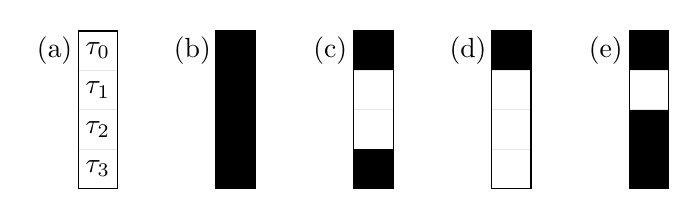
\begin{tikzpicture}[x=0.5cm, y=0.5cm] % {{{
\pgfmathsetmacro{\unitstep}{3.5}
% Coordenadas   {{{
\node at (-0.6,0.5) {(a)} ;
\draw[black!10] (0,0) rectangle (1,1); \node at (0.5,0.5) {$\tau_0$} ;
\begin{scope}[shift={(0,-1)}]
\draw[black!10] (0,0) rectangle (1,1); \node at (0.5,0.5) {$\tau_1$} ;
\end{scope}
\begin{scope}[shift={(0,-2)}]
\draw[black!10] (0,0) rectangle (1,1); \node at (0.5,0.5) {$\tau_2$} ;
\end{scope}
\begin{scope}[shift={(0,-3)}]
\draw[black!10] (0,0) rectangle (1,1); \node at (0.5,0.5) {$\tau_3$} ;
\end{scope} 
\draw (0,-3) rectangle (1,1); 
% }}}
\begin{scope}[shift={(1*\unitstep,0)}] % Identity {{{
% \begin{scope}[shift={(\unitstep*2,0)}]
\node at (-0.6,0.5) {(b)} ;
\fill[black] (0,0) rectangle (1,1);
\draw[black!10] (0,0) rectangle (1,1);
\begin{scope}[shift={(0,-1)}] \draw[black!10] (0,0) rectangle (1,1); \end{scope}
\begin{scope}[shift={(0,-2)}] \draw[black!10] (0,0) rectangle (1,1); \end{scope}
\begin{scope}[shift={(0,-3)}] \draw[black!10] (0,0) rectangle (1,1); \end{scope}
\draw (0,-3) rectangle (1,1); 
\begin{scope}[shift={(0,-1)}] \fill[black] (0,0) rectangle (1,1); \end{scope}
\begin{scope}[shift={(0,-2)}] \fill[black] (0,0) rectangle (1,1); \end{scope}
\begin{scope}[shift={(0,-3)}] \fill[black] (0,0) rectangle (1,1); \end{scope}
\end{scope} % }}}
\begin{scope}[shift={(2*\unitstep,0)}] % Dephasing {{{
\node at (-0.6,0.5) {(c)} ;
\fill[black] (0,0) rectangle (1,1);
% \draw (0,0) rectangle (1,1);
\draw[black!10] (0,0) rectangle (1,1);
\begin{scope}[shift={(0,-1)}] \draw[black!10] (0,0) rectangle (1,1); \end{scope}
\begin{scope}[shift={(0,-2)}] \draw[black!10] (0,0) rectangle (1,1); \end{scope}
\begin{scope}[shift={(0,-3)}] \draw[black!10] (0,0) rectangle (1,1); \end{scope}
\draw (0,-3) rectangle (1,1); 
% \begin{scope}[shift={(0,-1)}] \fill[black] (0,0) rectangle (1,1); \end{scope}
% \begin{scope}[shift={(0,-1)}] \draw (0,0) rectangle (1,1); \end{scope}
% \begin{scope}[shift={(0,-2)}] \fill[black] (0,0) rectangle (1,1); \end{scope}
% \begin{scope}[shift={(0,-2)}] \draw (0,0) rectangle (1,1); \end{scope}
\begin{scope}[shift={(0,-3)}] \fill[black] (0,0) rectangle (1,1); \end{scope}
% \begin{scope}[shift={(0,-3)}] \draw (0,0) rectangle (1,1); \end{scope}
\end{scope} % }}}
\begin{scope}[shift={(3*\unitstep,0)}] % Depolarization {{{
\node at (-0.6,0.5) {(d)} ;
\fill[black] (0,0) rectangle (1,1);
% \draw (0,0) rectangle (1,1);
\draw[black!10] (0,0) rectangle (1,1);
\begin{scope}[shift={(0,-1)}] \draw[black!10] (0,0) rectangle (1,1); \end{scope}
\begin{scope}[shift={(0,-2)}] \draw[black!10] (0,0) rectangle (1,1); \end{scope}
\begin{scope}[shift={(0,-3)}] \draw[black!10] (0,0) rectangle (1,1); \end{scope}
\draw (0,-3) rectangle (1,1); 
% \begin{scope}[shift={(0,-1)}] \fill[black] (0,0) rectangle (1,1); \end{scope}
% \begin{scope}[shift={(0,-1)}] \draw (0,0) rectangle (1,1); \end{scope}
% \begin{scope}[shift={(0,-2)}] \fill[black] (0,0) rectangle (1,1); \end{scope}
% \begin{scope}[shift={(0,-2)}] \draw (0,0) rectangle (1,1); \end{scope}
% \begin{scope}[shift={(0,-3)}] \fill[black] (0,0) rectangle (1,1); \end{scope}
% \begin{scope}[shift={(0,-3)}] \draw (0,0) rectangle (1,1); \end{scope}
\end{scope} % }}}
\begin{scope}[shift={(4*\unitstep,0)}] % (e) canal malo {{{
\node at (-0.6,0.5) {(e)} ;
\fill[black] (0,0) rectangle (1,1);
% \draw (0,0) rectangle (1,1);
\draw[black!10] (0,0) rectangle (1,1);
\begin{scope}[shift={(0,-1)}] \draw[black!10] (0,0) rectangle (1,1); \end{scope}
\begin{scope}[shift={(0,-2)}] \draw[black!10] (0,0) rectangle (1,1); \end{scope}
\begin{scope}[shift={(0,-3)}] \draw[black!10] (0,0) rectangle (1,1); \end{scope}
% \begin{scope}[shift={(0,-1)}] \fill[black] (0,0) rectangle (1,1); \end{scope}
% \begin{scope}[shift={(0,-1)}] \draw (0,0) rectangle (1,1); \end{scope}
\begin{scope}[shift={(0,-2)}] \fill[black] (0,0) rectangle (1,1); \end{scope}
% \begin{scope}[shift={(0,-2)}] \draw (0,0) rectangle (1,1); \end{scope}
\begin{scope}[shift={(0,-3)}] \fill[black] (0,0) rectangle (1,1); \end{scope}
% \begin{scope}[shift={(0,-3)}] \draw (0,0) rectangle (1,1); \end{scope}
\draw (0,-3) rectangle (1,1); 
\end{scope} % }}}
\end{tikzpicture} % }}}
\end{center}
	\caption{In (a) we introduce the positions of the single 
qubit diagrams, so that each square corresponds to a single 
$\tau_{\alpha}$, $\alpha=0,1,2,3$. The diagrams in 
(b), (c) and (d) correspond to the identity map, dephasing channel, and 
total depolarization, respectively. In (e) we show a map that only erases the component
$r_1$ and thus does not correspond to a quantum operation.}
	\label{fig:one:qubit:examples}
\end{figure} % }}}

\begin{figure} % {{{
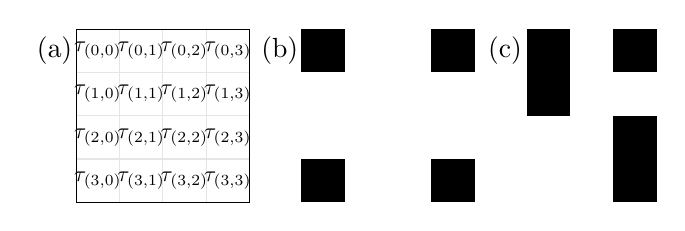
\begin{tikzpicture}[x=0.55cm, y=0.55cm] % {{{
\pgfmathsetmacro{\unitstep}{5.2}
\begin{scope}[shift={(0*\unitstep,0)}] % Coordenadas {{{
\node at (-0.5,0.5) {(a)} ;
% \cuadritotikz{}
    \foreach \x in {0,1,2,3} {
      \foreach \y in {0,1,2,3} {
        \begin{scope}[shift={(\x,-\y)}] 
          \draw[black!10] (0,0) rectangle (1,1); 
%           \draw (0,0) rectangle (1,1); 
          \node at (0.5,0.5) {\scalebox{.8}{$\tau_{(\y,\x)}$}};
         \end{scope}
%         \node at (0,-\y) (input\y) {$i_\y$};
%         \node[block] at (2,-\y) (block\y) {$f_\y$};
%         \draw[->] (input\y) -- (block\y);
%         \draw[->] (block\y.east) -- +(0.5,0);
    }
    }
 \draw (0,-3) rectangle (4,1);
\end{scope} % }}}
\begin{scope}[shift={(1*\unitstep,0)}] % Good channel {{{
\node at (-0.5,0.5) {(b)} ;
\cuadritotikz{}
%     \foreach \x in {0,1,2,3} {
%       \foreach \y in {0,1,2,3} {
%         \begin{scope}[shift={(\x,-\y)}] 
%           \draw (0,0) rectangle (1,1); 
% %           \node at (0.5,0.5) {$\tau_{\y,\x}$};
%          \end{scope}
% %         \node at (0,-\y) (input\y) {$i_\y$};
% %         \node[block] at (2,-\y) (block\y) {$f_\y$};
% %         \draw[->] (input\y) -- (block\y);
% %         \draw[->] (block\y.east) -- +(0.5,0);
%     }
%     }
\begin{scope}[shift={(0,-3)}] \fill[black] (0,0) rectangle (1,1); \end{scope}
\begin{scope}[shift={(3,-3)}] \fill[black] (0,0) rectangle (1,1); \end{scope}
\begin{scope}[shift={(0,0)}] \fill[black] (0,0) rectangle (1,1); \end{scope}
\begin{scope}[shift={(3,0)}] \fill[black] (0,0) rectangle (1,1); \end{scope}
\end{scope} % }}}
\begin{scope}[shift={(2*\unitstep,0)}] % Good channel {{{
\node at (-0.5,0.5) {(c)} ;
\cuadritotikz{}
%     \foreach \x in {0,1,2,3} {
%       \foreach \y in {0,1,2,3} {
%         \begin{scope}[shift={(\x,-\y)}] 
%           \draw (0,0) rectangle (1,1); 
% %           \node at (0.5,0.5) {$\tau_{\y,\x}$};
%          \end{scope}
% %         \node at (0,-\y) (input\y) {$i_\y$};
% %         \node[block] at (2,-\y) (block\y) {$f_\y$};
% %         \draw[->] (input\y) -- (block\y);
% %         \draw[->] (block\y.east) -- +(0.5,0);
%     }
%     }
\begin{scope}[shift={(0,0)}] \fill[black] (0,0) rectangle (1,1); \end{scope}
\begin{scope}[shift={(0,-1)}] \fill[black] (0,0) rectangle (1,1); \end{scope}
\begin{scope}[shift={(2,0)}] \fill[black] (0,0) rectangle (1,1); \end{scope}
\begin{scope}[shift={(2,-2)}] \fill[black] (0,0) rectangle (1,1); \end{scope}
\begin{scope}[shift={(2,-3)}] \fill[black] (0,0) rectangle (1,1); \end{scope}
\end{scope} % }}}
\end{tikzpicture} % }}}
	\caption{In (a) we introduce the
positions of two qubit diagrams. The diagrams in 
(b) corresponds to a quantum channel that results from the tensor product of
bit flip channels in each qubit [see \fref{fig:one:qubit:examples}(c)],
and in (c) a diagram of a map that is not a quantum channel is presented.}
	\label{fig:two:qubit:examples}
\end{figure} % }}}

% In \Fref{fig:PCE_figs} we introduce a pictorial representation of PCE operations of 
% 1, 2 and 3 qubits. Every position in the column, board or cube is associated with 
% the subindices of $\taus$ of a PCE operation. If a little square or cube  in position
% $\alpha_1,\ldots,\alpha_N$ is black, then $\taus=1$, if it is white, then $\taus=0$. For example,
% \begin{center}
% 
\includegraphics[width=2cm]{2qubits_pce_example}
% \end{center}
% this represents a PCE operation of 2 qubits that leaves invariant the Pauli 
% components $r_{0,0}$, $r_{0,2}$, $r_{1,0}$, $r_{2,2}$, $r_{3,2}$. This operation
% is not completely positive and therefore is not a quantum channel. In contrast, 
% \begin{center}
% \includegraphics[width=2cm]{2qubits_pceChannel_example01}
% \end{center}
% this other example of PCE operation that leaves invariant Pauli components 
% $r_{0,0}$, $r_{1,2}$, $r_{2,1}$, $r_{3,3}$ satisfies complete positivity and 
% is a quantum channel. 
% 
% 



% }}}





\section{Mathematical derivation} % {{{

{Vector space, mathematical derivation of properties}

\begin{itemize}
\item Diagonalización de la matriz de Choi de los canales de Pauli, es decir prueba da la $a$
\item Prueba de que la a diagonaliza \afnote{Breve descripción de detalles importantes. Cálculos en un Apéndice?}
\item Canales PCE como espacios vectoriales
\item Regla de $2^k$
\item Tamaño de las diferentes clases que borran un numero fijo de componentes
y tambien nota de qeu son igual entre complementarios: computo del numero de bases dada una dimension de subespacios vectoriales, aqui entra la formula del binomial-q.
\item Intento de identificar elementos, aka hermanistos PCE \cpnote{Esto dependerá de si sale algo interesante,}: De entrada aqui se tiene que mencionar minimo la identificacion del tamaño de las clases.
\item \ddnote{Agrego esto:} A final remarks of the derivation as a tool. Concepts might be complicated, but the tool gives some simple rules to the reader: \textit{tell me what components you want to keep, and the (vector) summation rules will give you the rest of components to make the target operation a CPTP one.}
\end{itemize}

% }}}
\section{Generators} % {{{
%\todo{Francois escribe una primera version del primer punto, y luego quizá Jose
%Alfredo o Carlos la terminan}

We now discuss the existence of a generator set for all PCE quantum channels, 
how to label each of them uniquely as $\pceg$ according to its local action 
on every qubit in the system, and, finally, we will discuss a symmetry of
both PCE quantum channel generators and $A$, the matrix that diagonalizes
the Choi matrix $\mcD_N$ of a PCE map.

There exists a subset of PCE quantum channels that generates the entire set; 
the nature of these generators may be studied, as we
shall see, with the properties of the aforementioned vector space.
By standard theorems of linear algebra, any proper subspace $W$, see \Eref{eq:19}, 
can be extended to a maximal non-trivial subspace of dimension $2N-1$ by
adjoining appropriate additional basis elements. This can be done in
different ways. We therefore arrive to the set of maximal extensions of $W$,
where every maximal subspace corresponds to a PCE quantum channel that
preserves half of the Pauli components. The intersection of all the elements of
this set reduces to $W$ itself,
and since intersection of subspaces translates to composition of PCE channels,
this implies that all PCE quantum channels can be obtained as
compositions of PCE channels corresponding to maximally non-trivial subspaces, plus
the identity map. In other words, the set of PCE quantum channels that preserve half 
of the components plus the identity map, are a generator set for 
all PCE channels.
Consider \Fref{fig:examplesPCE}; subfigures (c), (d) and (e) represent nontrivial 
PCE generators and the composition of any two of them yield the PCE channel
corresponding to (b). 


PCE generators may be characterized by its local action on every qubit 
in the system. This action can be encoded using a vector index $\vec\alpha$, 
as in \eqref{eq:pauli_strings}, hence each of the different $4^N$ 
vector indices may be uniquely related to each of the PCE generators
and thus denoted as $\mcG_{\vec\alpha}$.
% \cpnote{
The proof is simplified if one uses the Kraus representation developed in 
\sref{sec:kraus}, so we postpone the demonstration to appendix \ref{sec:2_qubits}.
\janote{referir a fig 5} For single qubits, the identity corresponds to $\mcG_0$, shown in 
\fref{fig:one:qubit:examples}(b), whereas $\mcG_3$ is shown in in 
\fref{fig:one:qubit:examples}(c).
% }
The 2-qubits PCE generator represented in subfigure (c)
of \Fref{fig:examplesPCE} acts on the first qubit (first column) as mapping its
Bloch sphere to de $x$-axis, and on the second qubit (first row) acts an identity,
hence it is labeled $\mcG_{(1,0)}$.
See \Fref{fig:appex:twoQ_PCEGs} for the notation of all 2-qubit PCE generators.

A reflection symmetry is identified for both PCE generators $\pceg$ and
the matrix $A$ that diagonalizes the Choi matrix $\mcD_N$ of a PCE map\cpnote{Creo que aun 
no tenemos el link entre el generador y la matriz A}.
Consider the map $\Sigma^{(k)}$ that reflects an index $\valpha$ with 
respect to the $k$-th axis. This map leaves all components of $\valpha$
invariant, except the $k$-th component, which is transformed according to 
\begin{equation}
% \Sigma: 
0\mapsto3,\quad3\mapsto0,\quad1\mapsto2,\quad2\mapsto1. 
\label{eq:Sigma}
\end{equation}
% and the associated 
All $N$ maps have the following properties:
\begin{enumerate}
\item $\Sigma^{(k)}(\vec\alpha)\oplus \Sigma^{(k)}(\vec\beta)=\vec\alpha\oplus \vec\beta$.
\item $\Sigma^{(k)}(\vec\alpha)\neq\vec\alpha$.
\end{enumerate}
From the first property, we now obtain
\begin{equation}
\valpha=\Sigma^{(k)}(\valpha) \oplus \Sigma^{(k)}(\vec0), 
\label{eq:Sigma}
\end{equation}
which means that if $\Sigma^{(k)}(\vec0)$ belongs
to a channel then 
$\tau_\valpha = \tau_{\Sigma^{(k)}(\vec\alpha)}$, where we used 
the fact that for channels, the non-zero elements are closed
under $\oplus$. In other words, the components of a PCE channel
are symmetric under reflection over the $k$-th axis. \cpnote{Quizá 
referencia a algunas figuras}. Now consider the case in which 
 $\Sigma^{(k)}(\vec0)$ does not belong to generator. Then 
$\tau_\valpha \ne \tau_{\Sigma^{(k)}(\vec\alpha)}$, since
the case $\tau_\valpha = \tau_{\Sigma^{(k)}(\vec\alpha)}=1$
is forbidden due to \eref{eq:Sigma} and the case 
$\tau_\valpha = \tau_{\Sigma^{(k)}(\vec\alpha)}=0$ is also forbidden 
because for generators, the codimension of the associated vector space 
is 1. 


% 
% 
% The symmetry for a PCE generator $\pceg$ is encoded in the 
% $N$-dimensional array of all $\taus$. The Cartesian grid associated with it 
% is either symmetric or anti-symmetric under reflection of the 
% indices in the $k$-th position in $\vec\alpha$. 
% Consider the map
% \begin{equation}
% % \Sigma: 
% 0\mapsto3,\quad3\mapsto0,\quad1\mapsto2,\quad2\mapsto1
% \label{eq:Sigma}
% \end{equation}
% Indeed, any generator is a subspace containing half the elements of the full vector space.  
% Map \eref{eq:Sigma} applied to the $k$-th qubit has the following properties
% \begin{enumerate}
% \item $\Sigma(\vec\alpha)\oplus \Sigma(\vec\beta)=\vec\alpha\oplus \vec\beta$.
% \item $\Sigma(\vec\alpha)\neq\vec\alpha$
% \end{enumerate}
% From the first property, we now obtain
% \begin{equation}
% \vec\alpha=\Sigma(\vec\alpha) \oplus \Sigma(\vec0)
% \end{equation}
% We now see that, depending on whether $\Sigma(\vec0)$ belongs (respectively does not belong) to the generator,
% $\vec\alpha$ belongs to the generator if and only if $\Sigma(\vec\alpha)$ belongs (respectively does not belong) to the generator.  
% 

\janote{Aquí iría la prueva de la simetría de reflexión que está en el horno aún.}
For instance, see that the 2-qubit PCE generators 
$\mcG_{(1,0)}$, $\mcG_{(3,2)}$ and $\mcG_{(2,2)}$
represented in subfigures (c), (d) and (e) of \Fref{fig:two:qubit:examples}, 
respectively, are either symmetric or anti-symmetric under reflection with 
respect to lines that divide the diagram in half vertically and horizontally. 
The same symmetry is identified for the rows and columns of $A$ if one 
labels each position in a row or column $A^{(i)}$ as $A^{(i)}_{\vec\alpha}$.
\janote{Aquí habría que agregar la prueva de simetría para la $A$.}

\begin{figure} % {{{
\centering
\includegraphics[width=\columnwidth]{oneQ_PCEGs-crop}
\caption{Connection between rows and columns of $a$ and single qubit PCE generators.
The rows or columns of $a$ and the diagrams of the generators are either 
symmetric or anti-symmetric under reflection.
\janote{Propuesta de figura para mostrar que generadores 
y la a obedecen las mismas simetrías.}
}
\label{fig:A_and_PCEGs_connection}
\end{figure} % }}}

\ddnote{Tengo entendido que esto se queria probar usando las simetrias, esto ya esta probado en la secc V}
Given that both matrix $\san$ and PCE generators $\pceg$ have the same 
symmetries, it is worth pointing out that $\san$ (and thus $a$) [see \eref{eq:san}] 
encodes all the information of PCE generators $\pceg$ and, therefore, of all PCE quantum channels. 
From the tensor power of matrix $a$ one can infer the $\{\taus\}$ of a PCE
generator $\pceg$ by taking any row or column $A^{(i)}$ and mapping 
all entries with $-1$ to $0$. In \Fref{fig:A_and_PCEGs_connection} we illustrate
this connection between $a$ and single qubit PCE generators.
In \appref{sec:2_qubits} we illustrate this program for 2-qubits PCE channels.

\cpnote{Sienot que no tiene flujo. Quizá se le pueda dar flujo usando el final 
del primer parrafo}

- - - - - - - - - - - - - - - - - - - - - - - - - - - - - - - - - - - -

The set of all PCE quantum channels may be sorted in subsets, 
which we will call equivalence classes, whose
elements are equivalent via particle swaps and local-basis element
permutations. 
\janote{El párrafo que pretendía ser este tendrá que ir en otra parte. 
Aún hay que decidirlo con los demás.}

% }}}



\section{Kraus operators and decoherence} % {{{
\cpnote{HAcer esta seccion despues de que david ponga lo de decoherencia, 
para servirla bien}
% \todo{Carlos hace una version}

Furthermore, quantum channels enjoy the well-known \textit{Kraus
representation} (or operator-sum representation) which reads 
\begin{equation}
\mcE[\rho]=\sum_i K_i \rho
K_i^\dagger{},
\end{equation}
with $\sum_i K_i^\dagger{}K_i=\one$ (the trace-preserving condition)~\cite{Kraus1983}.

The Kraus operators of PCE channels provide an insight in the physical processes
that yield such channels. In this section we investigate and construct such 
operators and explore the corresponding processes. 


To study the Kraus operators corresponding to PCE, it is enough to study 
the ones corresponding to generators, as all PCEs commute and thus to get the 
Kraus operators of an arbitrary PCE, one can easily combine the Kraus
operators of its generators. 


% The Kraus operators corresponding to one single qubit PCEs are 
% $\{\openone/\sqrt2, \sigma_i/\sqrt2\}$,
% % \begin{equation}
% % \{\openone/\sqrt2, \sigma_i/\sqrt2\}
% % \label{eq:kraus:PCE}
% % \end{equation}
% corresponding to the operation that leaves the component $\sigma_i$
% invariant~\cite{nielsen_chuang_2011}.
Inspection of the Kraus operators of two qubit PCEG lead to
the ansatz that the Kraus operators for the generator of 
$\mcG_{\vec \alpha}$ is 
\begin{equation}
\left\{\frac{\openone}{\sqrt2}, \frac{\sigma_{\vec \alpha}}{\sqrt2}\right\}. 
% \left\{\openone/\sqrt2, \left(\bigotimes_{k=1}^N \sigma_{\alpha_k}\right)/\sqrt2\right\}. 
\label{eq:kraus:PCE}
\end{equation}
Indeed, the Kraus operators corresponding to one single qubit PCEs are 
$\{\openone/\sqrt2, \sigma_\alpha/\sqrt2\}$,
corresponding to the operation that leaves the component $\sigma_\alpha$
invariant~\cite{nielsen_chuang_2011}.

We shall first show that the aforementioned Kraus operators indeed produce a PCE. 
Notice that 
% \begin{equation}
$\sigma_\alpha \sigma_\beta \sigma_\alpha =a_{\alpha \beta} \sigma_\beta$,
% \label{}
% \end{equation}
which in turn imply that 
\begin{equation}
\sigma_{\vec \alpha} \sigma_{\vec \beta} \sigma_{\vec \alpha} 
=\san_{\vec \alpha \vec \beta} \sigma_{\vec \beta}.
\label{eq:sigma_property}
\end{equation}
\cpnote{This is the original $a$, not $H \otimes H$. See how to relate these
two matrices, or define a new $a$ and $A$} \ddnote{tengo entendido que nunca se define o redefine $a$ como $H \otimes H$, ni en el apendice, solo se dice que se intercambian para ciertos calculos. Creo que la notacion es segura.}
% with $a$ the matrix that appears in \eqref{eq:eigvals-PCE}. 
Next, consider the action of a channel with Kraus representation 
\eqref{eq:kraus:PCE} on an $N$ qubit system:
\begin{align}
\rho \mapsto &\frac{1}{2^N}\sum_{\vec \beta} r_{\vec \beta} \left( \frac{1}{2} \sigma_{\vec \beta} + \frac{1}{2} \sigma_{\vec \alpha} \sigma_{\vec \beta} \sigma_{\vec \alpha} \right)\nonumber \\
=&\frac{1}{2^N}\sum_{\vec \beta} r_{\vec \beta} \frac{1+A_{\vec \alpha \vec \beta}}{ 2}\sigma_{\vec \beta}
\end{align}
However, since $\san_{\vec \alpha \vec \beta} = \pm 1$, the channel characterized
by Kraus operators  \eref{eq:kraus:PCE} is a PCE channel\ddnote{agrego 'channel', aqui el PCE map si es por construccion un canal}. Moreover, One can notice that, 
except for the first row, half of the matrix elements of each row is $+1$ and 
half $-1$, which implies that the aforementioned channel is a PCEG. 

% We still have to show that except for $i_1=\cdots=i_n=0$, half of the numbers 
% $(1+\prod_k a^{i_k}_{j_k})/2=1$, or equivalently, half of $\prod_k a^{i_k}_{j_k}=1$. 
% Consider a particular $l$ such that $i_l \ne 0$. This will make half of 
% the $\prod_k a^{i_k}_{j_k}$ 1 and half $-1$ (for fixed $l$). This also implies 
% that half of the correlations of the density matrix are erased and half preserved 
% so the channel is a PCEG. 

Notice also that a different choice of $\vec \alpha$ in \eref{eq:kraus:PCE}
leads to different channels. This can be seen noticing that if two channels were
the same, this would imply that the matrix representation of the corresponding
superoperator of $\sigma_{\vec \alpha} \cdot \sigma_{\vec \alpha}$ \ddnote{en este punto me confundio bastante esta notacion, contrapropongo $\rho \mapsto \sigma_{\vec \alpha}\rho \sigma_{\vec \alpha}$, que es una notación que hemos venido usando.}
would have to be the same which is clearly false. Since there are $4^n$ different 
$\vec \alpha$, this implies that all PCEG (plus the identity map) are in one to 
one correspondence.  

\cpnote{We might have spoken about the notation of the generators and here we 
can add a sentence about it, but I will wait till JA writes his part.}
% Two remarks. (i) The notation that we develop with Jose Alfredo coincides with the 
% generator. This notation is based on the action on each individual qubit. (ii) Counting the
% number of generators here is trivial. It is simply $4^n-1$ as previously noticed 
% from other arguments. 

Any PCE channel can be seen as the fixed point of some decoherence process. We will show this first for PCEGs. Consider the following dynamical process that \textit{implements} the PCEG $\mcG_{\vec \alpha}$ when $t\to \infty$,
\begin{align}
\mcG_{\vec \alpha,t}[\rho]&=e^{- \gamma t} \rho + (1-e^{-\gamma t})\mcG_{\vec \alpha}[\rho]\nonumber \\
&=\frac{\left( 1+e^{- \gamma t} \right)}{2} \rho +\frac{\left( 1-e^{- \gamma t} \right)}{2} \sigma_{\vec \alpha} \rho \sigma_{\vec \alpha},
\end{align}
where $\gamma>0$. It is easy to prove that the family of channels $\mcG_{\vec \alpha, t}$ parametrized with $t \geq 0$ forms a one-parametric semigroup, \ie{} $\mcG_{\vec \alpha, t_1}\mcG_{\vec \alpha, t_2}=\mcG_{\vec \alpha, t_1+t_2}$, therefore $\mcG_{\vec \alpha, t}$ describes a dissipative time-homogeneous Markovian process, those are always characterized by some Lindblad generator~\cite{lindblad}. The Lindblad generator of $\mcG_{\vec \alpha, t}$, $\mcL_{\vec \alpha}$, can be obtained with the standard procedure,  
\begin{equation}
\mcL_{\vec \alpha}[\rho]=\left. \frac{d\mcG_{\vec \alpha,t}[\rho]}{dt}\right|_{t=0}=\frac{\gamma\left(\sigma_{\vec \alpha}\rho \sigma_{\vec \alpha} -\rho \right)}{2},
\end{equation}
where the unique Lindblad operator associated with the relaxation ratio $\gamma/2$ is simply $\sigma_{\vec \alpha}$.

Since PCEGs commute, we can describe easily any other PCE channel as a fixed point of a decoherence process. For them, the Lindblad generators are simply the sum of the Lindbladians of the corresponding generators. As an example, consider the channel depicted in \fref{fig:two:qubit:examples} b), it is equal to $\mcG_{(0,3)}\mcG_{(3,3)}$, therefore it is the fixed point of the dissipation process described with the following Lindbladian,
\begin{equation}
\mcL=\frac{\gamma_{(0,3)}\left(\sigma_{(0,3)}\rho\sigma_{(0,3)}-\rho \right)}{2}+\frac{\gamma_{(3,3)}\left(\sigma_{(3,3)}\rho\sigma_{(3,3)}-\rho \right)}{2},
\end{equation}
where $\gamma_{(0,3)}$ and $\gamma_{(3,3)}$ are positive and correspond to the Lindblad operators $\sigma_{(0,3)}$ and $\sigma_{(3,3)}$. Notice that such election of Lindblad operators is not unique, as the PCE channel described here is also equal to $\mcG_{(0,3)}\mcG_{(3,0)}$.

In addition to the implementation via decoherence processes, PCE channels can also be described with collision models [cita]. To see this, observe that PCEGs can always be implemented using an unitary over the system and an ancilla [Stinespring citation]. For any PCEG, a qubit can always be chosen as the ancilla, concretely,
\begin{equation}
\mcG_{\vec \alpha}[\rho]:=\tr_{\text{qubit}} \left( U_{\vec \alpha} \left(\rho\otimes \projj{0}\right) U^\dagger{}_{\vec \alpha} \right),
\end{equation}
where $\tr_{\text{qubit}}$ denotes partial trace over the ancillary qubit, with
\begin{align}
U_{\vec\alpha}\ket{\psi} \ket{0}:=\frac{1}{\sqrt{2}} \left( \ket{\psi} \ket{0}+\sigma_{\vec\alpha} \ket{\psi}\ket{1} \right),\\
U_{\vec\alpha}\ket{\psi} \ket{1}:=\frac{1}{\sqrt{2}} \left( \ket{\psi} \ket{0}-\sigma_{\vec\alpha} \ket{\psi}\ket{1} \right).
\label{eq:Nqubit_stinespring}
\end{align}
Therefore, any concatenation of PCEGs can be described as a collision model with as many collisions as generators needed. In fact, generators are described with one collision. For the general case, consider some PCE channel $\mcE$ generated with $\left\{ \mcG_{\vec \alpha_1}, \mcG_{\vec \alpha_2}, \dots, \mcG_{\vec \alpha_M} \right\}$. For this, we have an environment consisting of $M$ qubits initially in the state $\left( \projj{0} \right)^{\otimes M}$ (or equivalently, one qubit environment with the additional assumption that its state is erased and transformed again $\ket{0}$ after each collision). The collision with the $k\text{th}$ particle is described by $U_{\vec \alpha_k}$, which acts solely over the system and the $k\text{th}$ particle. Therefore $\mcE$ can be written as follows,
\begin{equation}
\mcE[\rho]=\tr_{\text{E}} \left( \left(U_{\vec \alpha_1} \dots U_{\vec \alpha_M}\right)\left( \rho \otimes \projj{0}^{\otimes M}\right) \left(U_{\vec \alpha_1} \dots U_{\vec \alpha_M} \right)^\dagger{} \right),
\end{equation}
where $\tr_{\text{E}}$ is the partial trace over the total of the ancillary qubits. Notice that as PCEGs commute, the order of the collisions can be changed, taking care also of the order of the partial traces.
$U_{\vec\alpha_M}U_{\vec\alpha_{M-1}}\dots U_{\vec\alpha_1}$
Described as the system \textit{colliding} with qubit particles
\begin{itemize}
\item Relate to decoherence, for PCEG
\item Play with non PCEG PCEs
\item Dependiendo de si sale algo bonito, podemos poner algun modelo en
particular para todos los canales (sistema central + ambiente). Seria de buscar
dilataciones sencillas y razonables por lo menos a los canales generadores.
\todo{Davalos lidera la discusión de ese punto, pero no escribe nada}
\end{itemize} 

\begin{equation}
\mcL_{\vec \alpha}[\Delta]:= \frac{\gamma}{2}\left( \sigma_{\vec\alpha} \Delta \sigma_{\vec\alpha} -\Delta \right).
\label{eq:Nqubit_semigroup}
\end{equation}


% }}}

\section{The set of decoherence channels} % {{{
\todo{Aun no comenzar a escribir hasta que sepamos qeu queremos decir (si es
que queremos decir algo}
\begin{itemize}
\item Aca creo qe pueden ser puntos extremos de ese conjunto de canales
\item El conjunto dentro del conjunto de todos los canales (puntos extremos)
\end{itemize}
% }}}

\section{Qudits} % {{{

\begin{itemize}
\item Discuss what happens with general $d$ level systems and why it does not work
\item 
Linealidad de los eigenvalores de la matriz de Choi en función de las
$\tau_{j_1\ldots,j_n}$ de canales `\textit{component erasing}' de qudits. 
\end{itemize}

Discuss what happens with general $(2^k)^{\otimes n}$ level systems and why it does work
% }}}
\section{Conclusions}
\label{sec:conclusions}
\todo{al final}
\ddnote{Avienten ideas en cualquier idioma de lo que quieren que venga en las conclusiones}
   
% Frase de David {{{
\ddnote{Agrego esto:} A final remarks of the derivation as a tool. Concepts
might be complicated, but the tool gives some simple rules to the reader:
\textit{tell me what components you want to keep, and the (vector) summation
rules will give you the rest of components to make the target operation a CPTP
one.} \janote{Me gusta esto que puso David, pero lo movería a las conclusiones.}
\par % }}}

% ideas{{{
\textcolor{jacolor}{
\begin{enumerate}
\item We introduced a novel type of Pauli maps: Pauli component erasing (PCE) maps.
PCE maps are operators that totally project the density matrix of a system on $N$ 
qubits onto subsets of elements of Pauli strings basis. PCE maps either
preserve or completely erase the projections of the density matrix 
onto the elements of Pauli strings basis. By construction, PCE maps are
trace-preserving. In Figs \ref{fig:one:qubit:examples} and 
\ref{fig:two:qubit:examples} we introduced diagrams to represent PCE maps
of 1 and 2 qubits. We were interested in investigating PCE maps 
that represent quantum physical evolutions, i.e., PCE maps that are
quantum channels. The problem is reduced to finding the conditions for
a PCE map to be completely positive.
\item We provided exact diagonalization for Pauli diagonal maps in general.
To evaluate the CP condition we evaluated the positivity of Choi matrix of
a PCE map, as established in the Choi-Jamiokolwsky isomorphism. Exact 
diagonalization shows a structure where the CP conditions of general 
Pauli diagonal maps are encoded in a matrix of 1 qubit.
\item We then restricted to PCE maps and investigated the algebraic structure
of PCE quantum channels. We showed that PCE quantum channels have an associated
vector space structure over the field of two elements $\{0,1\}$. 
From there, we derived all properties of PCE 
quantum channels. PCE quantum channels are not only characterized by the number
of Pauli components preserved but for the particular sets of components preserved too.
The coefficients of Pauli components must form a vector space.
\item We showed that PCE quantum channels posses generators, understood
as maximal vector subspaces. PCE quantum channels have symmetries. From
the vector structure it follows the existence of PCE generators as 
maximal non trivial subspaces. This PCE generatos have symmetries.
\item Kraus operators of PCE quantum channels are easy. They are the 
identity plus...
\item Physical implementation of PCE maps.
\end{enumerate} }
% }}}



\section{Ideas sueltas} % {{{
\subsection{Preguntas abiertas}
\begin{itemize}
\item \afnote{Clasificación de las clases de canales PCE: Entanglement breaking, divisible...}
\end{itemize}
% }}}
\par
\section*{Acknowledgments}
Support by projects CONACyT 285754 and UNAM-PAPIIT IG100518, IG101421 
is acknowledged. 
% Conversations with F. de Melo, T. H. Seligman, J. D. Urbina
% and A. Diaz-Ruelas are also acknowledged. 
\bibliographystyle{unsrt}
\bibliography{references}
\appendix
\section{Number of PCEs for a fixed number of invariant components} % {{{
\label{app:contar}
Finally, we may enumerate straightforwardly the subspaces $W$ of dimension $K$.
We do this in 2 steps: first, we evaluate $\nnn_{K,N}$, the number of all
linearly independent subsets $V$ with $K$ elements. Each of these is the basis
of one subspace of dimension $K$, but each subspace has a number $\mmm_K$ of
different bases. The crucial point is that $\mmm_K$ is independent of the
subspace under consideration: $\mmm_K$ simply describes the number of linear
maps of $W$ onto itself. The total number $\sss_{N,K}$ of subspaces of
dimension $K$ is therefore $\nnn_{N,K}/\mmm_K$. 

To evaluate $\nnn_{N,K}$ we proceed by steps: the first element of the basis
can be any non-zero element, of which the number is $2^{2N}-1$. For the  basis
element $m+1$, we must choose from those which do not belong to the $m$
dimensional space generated by the first $m$ basis elements, so that one
chooses from $2^{2N}-2^{m}$. We thus have
\begin{equation}
\nnn_{N,K}=\prod_{m=0}^{K-1}\left( 2^{2N}-2^{m} \right).
\label{eq.20}
\end{equation}
On the other hand, any map of a $K$-dimensional vector space $W$ onto itself is
uniquely defined by a non-singular binary $K\times K$ matrix over the field
$\{0,1\}$. To count these, we proceed as above: the first line is an arbitrary
non-zero vector, of which there are $2^K-1$. For the row $m+1$  we must choose
an arbitrary vector not belonging to those generated by the first $m$ vectors,
of which there are $2^K-2^{m}$.  This eventually yields
\begin{equation}
\mmm_{K}=\prod_{m=0}^{K-1}\left(
2^{K}-2^{m}
\right).
\label{eq.21}
\end{equation}
From this follows that
\begin{equation}
\sss_{N,K}=\prod_{m=0}^{K-1} \frac{2^{2N-m}-1}{2^{K-m}-1}.
\label{eq:22}
\end{equation}
%An elementary test is $N=3$ and $K=2,3$: 
%\begin{eqnarray}
%\sss_{3,2}&=&\frac{(2^6-1)(2^5-1)}{(2^2-1)(2^1-1)}=\frac{63\cdot31}{3}=651,\\
%\sss_{3,3}&=&\frac{(2^6-1)(2^5-1)(2^4-1)}{(2^3-1)(2^2-1)(2^1-1)}=\frac{63\cdot31\cdot15}{7\cdot3}=1395,
%\end{eqnarray}
%which are indeed the values found numerically. 
The following symmetry relation
\begin{equation}
\sss_{N,K}=\sss_{N,2N-K}
\end{equation}
can also be proved straightforwardly from (\ref{eq:22}).


% }}}
\end{document}
